
%(BEGIN_QUESTION)
% Copyright 2006, Tony R. Kuphaldt, released under the Creative Commons Attribution License (v 1.0)
% This means you may do almost anything with this work of mine, so long as you give me proper credit

Explain what the following ``ladder-logic'' circuit does, and identify the meaning of each symbol in the diagram:
Forklar funksjonen til dettte styrestrømsskjemaet. Skriv også opp navn på symboler og hva referansebetegnelsene står for. 

$$\includegraphics[width=15.5cm]{i00364x01.eps}$$

\vskip 20pt \vbox{\hrule \hbox{\strut \vrule{} {\bf Suggestions for Socratic discussion} \vrule} \hrule}

\begin{itemize}
\item{} Explain why the TSH uses a {\it normally-open} contact instead of a {\it normally-closed} contact.
\item{} Explain why the TSL uses a {\it normally-closed} contact instead of a {\it normally-open} contact.
\item{} Based on what we see in this diagram, determine whether the electric solenoid valve allows cooling water to flow when energized, or when de-energized.
\item{} What do the designations ``L1'' and ``L2'' refer to in ladder-logic electrical diagrams?
\item{} Suppose switch TSL has a trip setting of 105 $^{o}$F (falling) and a deadband value of 2 $^{o}$F.  Explain how this switch will respond to a rising and falling temperature.
\item{} Suppose we wished to have switch TSHH activate {\it two} different alarm lights instead of just one.  Modify the circuit diagram accordingly.
\end{itemize}

\underbar{file i00364}
%(END_QUESTION)





%(BEGIN_ANSWER)

This is an automatic cooling system with high and low temperature alarms.

%(END_ANSWER)





%(BEGIN_NOTES)











\vfil \eject

\noindent
{\bf Summary Quiz:}

Identify the most likely purpose of the process switch shown in the following schematic:

$$\includegraphics[width=15.5cm]{i00364x02.eps}$$

\begin{itemize}
\item{} Open a hot-water valve to prevent a machine from freezing
\vskip 5pt 
\item{} Regulate a reactor vessel at a controlled temperature setpoint
\vskip 5pt 
\item{} Sound an audible alarm if a reactor's temperature gets too low
\vskip 5pt 
\item{} Open a pressure-relief valve if an accumulator's pressure is too high
\vskip 5pt 
\item{} Open a cooling water valve to cool down an overheated machine
\vskip 5pt 
\item{} Open a make-up water valve if a cooling water reservoir falls empty
\end{itemize}

%INDEX% Measurement, temperature: switch

%(END_NOTES)


